\documentclass[12pt]{article}
\NeedsTeXFormat{LaTeX2e}

%%%%%%%%%%%%%%%%%%%%%%%%%%%%%%%%%%%%%%%%%

% Template by Nicholas Bertollo
% You may change and reuse this as you see fit

%%%%%%%%%%%%%%%%%%%%%%%%%%%%%%%%%%%%%%%%%

% Replace this information!
\newcommand{\studyunit}{MATH1064}
\newcommand{\studyperiod}{Semester 2, 2025}

%%%%%%%%%%%%%%%%%%%%%%%%%%%%%%%%%%%%%%%%%

\usepackage[svgnames]{xcolor}
\usepackage[T1]{fontenc}
\usepackage[margin=2.7cm,a4paper]{geometry}
\renewcommand{\baselinestretch}{1.15}

\usepackage[osf]{mathpazo}
\usepackage{amsmath,amsthm,amsfonts,amssymb,mathtools}

\usepackage{hyperref,url}
\usepackage{xstring}

\usepackage{environ}
\usepackage{tasks}

\usepackage{etoolbox}
\usepackage{fourier-orns}
\usepackage{kvoptions}
\usepackage[]{units}
% \usepackage[normal]{subfigure}
\usepackage{subfig}

% Algorithms package

% \usepackage[ruled]{algorithm2e} % You can use the algorithm2e if you'd like
\usepackage[noend]{algpseudocode} % You may get rid of noend if you like. 
\usepackage{algorithm}
\usepackage{algorithmicx}

% No indents
\usepackage[parfill]{parskip}

% Tikz diagrams
\usepackage{tikz}
\usetikzlibrary{shapes.geometric,patterns,patterns.meta,arrows,positioning,fit,calc}
\pgfdeclarelayer{background}
\pgfsetlayers{background,main}

% Graphics and images
\usepackage{graphicx}
\graphicspath{ {./images/} }

% Header
\usepackage{fancyhdr}
\addtolength{\headheight}{2.5pt}
\pagestyle{fancy}
\fancyhead{} 
\fancyhead[L]{\sc \studyunit}
\fancyhead[R]{\sc \studyperiod}
\fancyfoot{}
\fancyfoot[R]{\thepage}
\renewcommand{\headrulewidth}{0.75pt}

%%%%%%%%%%%%%%%%%%%%%%%%%%%%%%%%%%%%%%%%%%%%%%%%%%%%%%%%%%%%%%%%%%%%%%%%%%%%%%%%%%

% Some basic mathematics commands!

\DeclarePairedDelimiter\ceil{\lceil}{\rceil}
\DeclarePairedDelimiter\abs{\lvert}{\rvert}

\newcommand{\lt}{\ensuremath <}
\newcommand{\gt}{\ensuremath >}
\newcommand{\Z}{\mathbb{Z}}
\newcommand{\N}{\mathbb{N}}
\newcommand{\R}{\mathbb{R}}
\newcommand{\Q}{\mathbb{Q}}
\newcommand{\U}{\mathbb{U}}
\newcommand{\compline}[1]{\overline{#1}}
\newtheorem{theorem}{Theorem}
\theoremstyle{definition}
\newtheorem{definition}{Definition}

%%%%%%%%%%%%%%%%%%%%%%%%%%%%%%%%%%%%%%%%%%%%%%%%%%%%%%%%%%%%%%%%%%%%%%%%%%%%%%%%%%

% Macros
% \newcounter{weekcntr}
% \newcommand*{\week}{
%     \stepcounter{weekcntr}
%     \section{Week \theweekcntr}
% }
    
 
\begin{document}
    \begin{titlepage}
        \begin{center}
            \vspace*{1cm}

            \section*{MATH1064 Study Notes}

            \vspace{0.25cm}
            University of Sydney \\
            \studyperiod \\
            \studyunit

            \vfill
            \includegraphics{thumbs_up_emoji.png}
            \vspace{1.5cm}

            Happy studying!
            
       \vspace{0.8cm}
            
        \end{center}
    \end{titlepage}

    \tableofcontents
    
    \newpage
    \section{Introduction to Discrete Maths and Set Theory}
    \subsection{Introduction to Discrete Maths}

        Discrete maths is the study of "discrete structures", this includes objects which are:
        \begin{itemize}
            \item Countable or listable
            \item Distinct and unconnected.
        \end{itemize}

        There are two objectives of {\studyunit}:
        \begin{enumerate}
            \item Develop mathematical reasoning skills. This involves using \textbf{logic and proofs}, and 
            \textbf{rigorously} (exhausting all possibilities) finding solutions to problems.
            \item Study \textbf{discrete structures} and their properties including:
            \begin{itemize}
                \item Sets and functions
                \item Prime numbers and modular arithmetic
                \item Graphs and networks
                \item Counting and probability.
            \end{itemize}
        \end{enumerate}
    
        \subsection{Introduction to Set Theory}
        \subsubsection{Definitions}
        \begin{definition}[Set]
            \label{def:set}
            A \textbf{set} $S$ is a collection of objects, called \textbf{elements} of $S$.
        \end{definition}

        \begin{itemize}
                \item If $x$ is an element of $S$, $x \in S$
                \item If not, then $x \notin S$.
            \end{itemize}

        Sets can be finite or infinite:
        \begin{itemize}
            \item Example (finite): $S = \{2, 3, 5\}$
            \item Example (infinite): $S = \{0, 1, 2, \dots\} = \N$ \\
        \end{itemize}

        \begin{definition}[Set Equivalence]
            Two sets $S$ and $T$ are said to be equal if they contain the same elements, regardless of \textbf{order} or 
            \textbf{repetition}.
        \end{definition}

        \begin{itemize}
            \item Example 1: \\
            \begin{align*}
                S &= \{1,1,5,3\} \\
                T &= \{1,3,5\} \\
                S &= T
            \end{align*}
            \item Example 2:
            \begin{align*}
                S &= \{-1, 0, 1, \dots\} \\
                T &= \{0, 1, \dots\} \\
                S &\neq T
            \end{align*}
        \end{itemize}

        \begin{definition}[Empty Set]
            \label{def:empty-set}
            The \textbf{empty set} is a unique set containing no elements. $\emptyset = \{\}$.\\
        \end{definition}
        \begin{definition}[Singlton Set]
            \label{def:singleton-set}
            A \textbf{singleton set} has only one element, e.g. $S = \{x\}$ or $S = \{x, x, x\}$
        \end{definition}

        \subsubsection{Unpacking Sets}
        Sets can contain other sets as elements, inner sets are considered distinct elements even if 
        their contents are the same as other elements in the outer set. This is because when we unpack sets,
        we only remove outer curly braces \{ \}.
        \begin{align*}
            S &= \{1, 2, \{1\} \} \\
            \abs{S} &= 3 \text{ distinct elements}
        \end{align*}

        \subsubsection{Sets with Properties}
        We can describe sets using \textbf{set builder notion} which indicates the properties of a set.
        \begin{align*}
            A = \{x \in S \mid P(x) \}
        \end{align*}
        "The set A consists of all elements $x$ of $S$ such that $x$ has property $P$".\\\\
        Examples:
            \begin{align*}
                \{x \in \N \mid 3 \le x \le 5\} &= \{3,4,5\} \\
                \{y \in \Z \mid y=2k \text{ for some } k \in \Z\} &= \{\dots, -2, 0, 2, \dots\} \\
                \{2z + 1 \mid z \in \N\} &= \{1, 3, 5, \dots\}
            \end{align*}
        
            \subsubsection{Russel's Paradox}
            Define a set $T = \{S, set \mid S \notin S\}$. The set $T$ contains any set $S$ which does not contain itself.
            
            Consider if $T \in T$:
            \begin{itemize}
                \item If $T \in T$: $T$ does not satisfy the condition.
                \item If $T \notin T$: $T$ does satisfy the condition, thus $T \in T$ according to our definition.
            \end{itemize}
            This induces a contradiction, hence demonstrating that we need \textbf{axioms} which \textbf{rigorously} state
            how to define and build sets.
        
            \subsubsection{Operations on Sets}
            \begin{definition}[Union]
                \label{def:union}
                Given two sets $S$ and $T$, the \textbf{union} of $S$ and $T$ is the set containing all elements from $S$ and $T$.
                This is written as $S \cup T$ where $x \in S$ \textbf{OR} $x \in T$.
            \end{definition}
            \begin{itemize}
                \item Example 1: $\{1,2,3\} \cup \{2,5\} = \{1,2,3,5\}$
                \item Example 2: $\{0,1,2,\dots\} \cup \{0,-1,-2,\dots\} = \Z$ \\
            \end{itemize}

            \begin{definition}[Intersection]
                \label{def:intersection}
                Given two sets $S$ and $T$, the \textbf{intersection} of $S$ and $T$ is the set of elements belonging to
                both $S$ and $T$. This is written as $S \cap T$ where $x \in S$ \textbf{AND} $x \in T$.
            \end{definition}
            \begin{itemize}
                \item Example 1: $\{1,2,3\} \cap \{2,5\} = \{2\}$
                \item Example 2: $\{1,2,3,\dots\} \cap \{-1,-2,-3,\dots\} = \emptyset$ \\
            \end{itemize}

            Multiple unions and intersections can be taken at a time.
            \begin{align*}
                \displaystyle\bigcup_{i=1}^{3} \{i, 2i\} &= \{1,2\} \cup \{2,4\} \cup \{3,6\} \\
                &= \{1,2,3,4,6\}
            \end{align*}
            \begin{align*}
                \displaystyle\bigcap_{i=1}^{3} \{i, i+1, i+2\} &= \{1,2,3\} \cap \{2,3,4\} \cap \{3,4,5\} \\
                &=\{3\}
            \end{align*}
            
            Formally, for sets $A_1,A_2,\dots,A_i$ we define the set $A_i$ as:
            \begin{equation*}
                \displaystyle\bigcup_{i=1}^{\infty} A_i = \{x \mid x \in A_{k} \text{ for SOME } k \ge 1\}
            \end{equation*}
            That is for an infinite series of unions, $x$ is an element that appears \textbf{at least once} 
            in the sets $A_k$ for $k \ge 1$.

            And similarly for intersections, we define the set $A_i$ as:
            \begin{equation*}
                \displaystyle\bigcap_{i=1}^{\infty} A_i = \{x \mid x \in A_{k} \text{ for ALL } k \ge 1\}
            \end{equation*}
            That is, for an infinite series of intersections, $x$ is an element which appears in \textbf{all} 
            sets $A_k$ for $k \ge 1$.

            
            \subsubsection{Subsets}
            \begin{definition}[Subsets]
                \label{def:subset}
                A set $S$ is a \textbf{subset} of another set $T$ if every element of $S$ is an element of $T$. This
                is written as $S \subset T$.
            \end{definition}

            Additionally, if $S$ is a subset of $T$ but is not equal to $T$, then it is considered a \textbf{proper subset},
            denoted as $S \subseteq T$.
            
            For example,
            \begin{align*}
                S &= \{2,4,6\} \\
                T &= \{2,4,6,8\}\\
                S &\subseteq T, \text{ since $8 \notin S$}
            \end{align*}


            \subsubsection{Proving Subset Relationships}
            To prove $S \subseteq T$, we need to:
            \begin{enumerate}
                \item Take an arbitrary element of $S$, which we  call $x$
                \item Show that $x \in T$ \\
            \end{enumerate}

            \textbf{Example:} Let $S$ and $T$ be sets where,
            \begin{align*}
                S &= \{2n \mid n \in \N, n \ge 1\} \\
                T &= \{2^{m} \mid m \in \N\}
            \end{align*}
            \begin{proof}
                Let $x \in S$, by definition $x=2^n$ for some $n \ge 1$.
                \begin{align*}
                    x &=2^n \\
                    x &=2(2^{n-1}), \text{ rewriting $x$}
                \end{align*}
                Since $n \ge 1$, $n-1 \ge 0$ meaning that $n-1 \in \N$ $\implies 2^{n-1} \in \N$.
                Because $2^{n-1}$ is a natural number, we can rewrite $x = 2m$ where $m=2^{n-1}$ as we know
                $m \in \N$, $x \in T \implies S \subseteq T$.
            \end{proof}

            \subsubsection{Proving Equality Relationships}
            To prove that $S=T$, we need a \textbf{"double containment proof"} which shows that both sets have the same
            elements, that is:
            \begin{enumerate}
                \item Every $x \in S$ also satisifes $x \in T$
                \item Every $x \in T$ also satisfies $x \in S$
            \end{enumerate}
            \textbf{Example:} Let $S$ and $T$ be sets where,
            \begin{align*}
                S &= \{2m+1 \mid m \in \Z\} \\
                T &= \{2r-1 \mid r \in \Z\}
            \end{align*}
            \begin{proof}[Proof. Show $S \subseteq T$]
                Let $x \in S$, then $x = 2m+1$ for some $m \in Z$. \\
                Let $r = m+1$.
                \begin{align*}
                    x &= 2m + 1 \\
                    x &= 2m + 2 - 1, \text{ rewriting $x$} \\
                    x &= 2(m + 1) - 1, \text{ notice $m+1 = r$} \\
                    x &= 2r - 1, \text{this is the same as $x \in T$}
                \end{align*}
                $x = 2r -1$ for some $r \in \Z$. Thus, $x \in T \implies S \subseteq T$.
            \end{proof}

            \begin{proof}[Proof. Show $T \subset S$]
                Let $x \in T$, then $x = 2r-1$ for some $r \in \Z$. \\
                Let $m = r - 1$.
                \begin{align*}
                    x &= 2r-1 \\
                    x &= 2r - 2 + 1 \\
                    x &= 2(r-1) + 1 \\
                    x &= 2m + 1
                \end{align*}
                $x = 2m + 1$ for some $m \in \Z$. Thus, $x \in S \implies T \subseteq T$.
            \end{proof}
            Since $S \subseteq T$ and $T \subseteq S$, the two sets must have the same elements and are equal, $S = T$.


            \subsection{More Set Theory}
            \subsubsection{Cardinality}
            The \textbf{cardinality} of a set $S$ in a rough sense refers to the size of $S$, i.e. the no. of elements in
            $S$.
            \begin{itemize}
                \item If $S$ is finite, then $\abs{S}$ is the number of distinct elements in $S$.
                \item If $S$ is infinite, then we write $\abs{S} = \infty$. 
            \end{itemize}
            Note that there can be \textbf{different infinite cardinalities}, or sizes of infinities. A basic example of this
            is the set of natural numbers $\N$ compared to the set of real numbers $\R$.

            \subsubsection{Set Differences}
            \begin{definition}[Set Difference]
                \label{def:set-difference}
                Given two sets $S$ and $T$, the \textbf{set difference} is the set of elements $x \in S$ and $x \notin S$.
                This is written as $S \backslash T$ or $S - T$.
            \end{definition}
            \begin{itemize}
                \item Example 1: $\{1,2,3\}\backslash \{2, 5\} = \{1, 3\}$
                \item Example 2: $\{0, 1, 2, \dots\} \backslash \{0, -1, -2, \dots\} = \{1, 2, \dots\}$
                \item Example 3: $\N \backslash \Z = \emptyset$
            \end{itemize}

            \subsubsection{Universal Set}
            \begin{definition}[Universal Set]
                \label{def:universal-set}
                Let $\U$ be some \textbf{universal set} which is the set containing all elements of which other sets are
                subsets. The universal set is context dependent.
            \end{definition}
            \begin{itemize}
                \item $\U = \Z$, if working with number theory
                \item $\U = \R^2$, if working with plane geometry
            \end{itemize}

            \subsubsection{Complementary Set}
            \begin{definition}[Complement]
                \label{def:complement}
                For a set $S \subseteq \U$, the \textbf{complement} of $S \in \U$ is given by $x \in \U$ where\
                $x \notin S$. This is written as $\compline{S}$ or $S^{\complement}$.
            \end{definition}
            In other words, $\compline{S}$ is the set containing all elements not in $S$, where the range of elements
            considered is constrained by $\U$. This resolves the Russel Paradox.

            For example, if $\U = \Z$:
            \begin{itemize}
                \item $\compline{\{1,2,3\}} = \{\dots, -1, 0, 4, \dots\}$
                \item $\compline{\{x \in \Z \mid x \gt 0\}} = \{x \in \Z \mid x \lt 0\}$
                \item $\compline{\Z} = \emptyset$
            \end{itemize}

            \subsubsection{Venn Diagrams}
            \textbf{Venn Diagrams} are tools used to visualise relationships between sets.

            \def\circleA{(0,0) circle (1.5cm)}
            \def\circleB{(0:2cm) circle (1.5cm)}
            \def\rectangle1{(-2,-2) rectangle (4,2)}
            \colorlet{circle edge}{black!50}
            \colorlet{circle area}{black!20}
            \tikzset{filled/.style={fill=circle area, draw=circle edge, thick},
            outline/.style={draw=circle edge, thick}}

            \setlength{\parskip}{5mm}
            \begin{figure}[hbt!]
            \centering
            \subfloat{
                \begin{tikzpicture}
                    \begin{scope}
                        \draw \rectangle1;
                        \clip \circleA;
                        \draw[pattern=north west lines] \circleB;
                    \end{scope}
                    \draw[outline] \circleA node {$A$};
                    \draw[outline] \circleB node {$B$};
                    \node[anchor=south] at (current bounding box.north) {$A \cap B$};
                \end{tikzpicture}
            }
            \hspace{50px}
            \subfloat{
                \begin{tikzpicture}
                    \begin{scope}
                        \draw \rectangle1;
                        \draw[pattern= north west lines] \circleA;
                        \draw[pattern= north west lines] \circleB;
                    \end{scope}
                    \draw[outline] \circleA node {$A$};
                    \draw[outline] \circleB node {$B$};
                    \node[anchor=south] at (current bounding box.north) {$A \cup B$};
                \end{tikzpicture}
            }
            \vspace{10px}
            \subfloat{
                \begin{tikzpicture}
                    \begin{scope}
                        \draw \rectangle1;
                        \draw[pattern= north west lines] \circleA;
                        \draw[pattern= north west lines, fill=white] \circleB;
                    \end{scope}
                    \draw[outline] \circleA node {$A$};
                    \draw[outline] \circleB node {$B$};
                    \node[anchor=south] at (current bounding box.north) {$A \backslash B$};
                \end{tikzpicture}
            }
            \hspace{50px}
            \subfloat{
                \begin{tikzpicture}
                    \begin{scope}
                        \draw[pattern= north west lines] \rectangle1;
                        \draw[outline, fill=white] \circleA;
                        \draw[outline, fill=white] \circleB;
                    \end{scope}
                    \draw[outline] \circleA node {$A$};
                    \draw[outline] \circleB node {$B$};
                    \node[anchor=south] at (current bounding box.north) {$\compline{A \cup B}$};
                \end{tikzpicture}
            }
            \end{figure}

            Venn diagrams are useful for intuition and can be used to guide proofs, but are not sufficient as rigorous proofs in
            of themselves.

            \textbf{Example:} Prove if $A \cap (B \cup C) = (A \cap B) \cup (A \cap C)$

            \def\circleC{(1,-1.5) circle (1.5cm)}
            \def\rectangle2{(-2,-3.5) rectangle (4,2)}

            \setlength{\parskip}{5mm}
            \begin{figure}[hbt!]
            \centering
            \subfloat{
                \begin{tikzpicture}
                    \begin{scope}
                        \draw \rectangle2;
                        \clip \circleB \circleC;
                        \draw[pattern= north west lines] \circleA;
                    \end{scope}
                    \draw[anchor=south, outline] \circleA node {$A$};
                    \draw[anchor=south, outline] \circleB node {$B$};
                    \draw[anchor=north, outline] \circleC node {$C$};
                    \node[anchor=south] at (current bounding box.north) {$A \cap (B \cup C)$};
                \end{tikzpicture}
            }
            \hspace{50px}
            \subfloat{
                \begin{tikzpicture}
                    \begin{scope}
                        \draw \rectangle2;
                        \draw \rectangle2;
                        \clip \circleB \circleC;
                        \draw[pattern=north west lines] \circleA;
                    \end{scope}
                    \draw[anchor=south, outline] \circleA node {$A$};
                    \draw[anchor=south, outline] \circleB node {$B$};
                    \draw[anchor=north, outline] \circleC node {$C$};
                    \node[anchor=south] at (current bounding box.north) {$(A \cap B) \cup (A \cap C)$};
                \end{tikzpicture}
            }
            \end{figure}

            \begin{proof}[Proof. Double Containment]
                First, show $A \cap (B \cup C) \subseteq (A \cap B) \cup (A \cap C)$. \\
                Let $x \in A \cap (B \cup C)$:
                \begin{align*}
                    \text{Then $x \in A$ and $x \in (B \cup C)$} \\
                    x \in (B \cup C) \implies x \in B \text{ or } x \in C \\
                    \text{if $x \in B$}, x \in (A \cap B) \implies x \in (A \cap B) \cup (A \cap C) \\
                    \text{if $x \in C$}, x \in (A \cap C) \implies x \in (A \cap C) \cup (A \cap B) \\
                    \implies A \cup  (B \cap C) \subseteq (A \cap B) \cup (A \cap C)
                \end{align*}

                This proof works because we know that if $x \in (A \cap B)$, then suppose we expand the set ($A \cap B$) by
                including another arbitrary set, say $(A \cap C)$. We can implicitly assume $x$ is an element of $(A \cap B) \cup (A \cap C)$
                since we are simply expanding the scope of the set.

                Second, show $(A \cap B) \cup (A \cap C) \subseteq A \cap (B \cup C)$. \\
                Let $x \in (A \cap B) \cup (A \cap C)$:

                \begin{align*}
                    \text{Then $x \in A$ and $x \in B$} \\
                    \implies x \in (B \cup C) \\
                    \implies x \in A \cap (B \cup C) \\
                \end{align*}
                \begin{align*}
                    \text{Then $x \in A$ and $x \in C$} \\
                    \implies x \in (C \cup B) \\
                    \implies x \in A \cap (C \cup B)
                \end{align*}
                
                Thus, $(A \cap B) \cup (A \cap C) \subseteq A \cap (B \cup C)$, indicating that both sets are equal.

            \end{proof}

            \subsubsection{Set Identities}
            \begin{itemize}
                \item $A \cap (B \cup C) = (A \cap B) \cup (A \cap C)$
                \item $A \cup (B \cap C) = (A \cup B) \cap (A \cup C)$
                \item $\compline{A \cap B} = \compline{A} \cup \compline{B}$
                \item $A \cap (A \cup B) = A$
            \end{itemize}

    \newpage
    \section{Week 2}
    \subsection{Power Sets and Cartesian Planes}
    \subsubsection{Power Set}
    \begin{definition}[Power Set]
        \label{power-set}
        For a set $S$ the \textbf{power set} of $S$ is the set which contains all possible
        subsets of $S$. This is denoted as $P(S) = \{A \mid A \subseteq S\}$.
    \end{definition}
    For example,
    \begin{itemize}
        \item $S = \{a, b\} \implies P(S) = \{\emptyset, \{a\}, \{b\}, \{a,b\}\}$
        \item $S = \emptyset \implies P(S) = \{\emptyset\}$
        \item $S = \{1,2,3\} \implies P(S) = \{\emptyset, \{1\},\{2\},\{3\},\{1,2\},\{1,3\}, \{2,3\},\{1,2,3\}\}$ \\
    \end{itemize}

    \begin{theorem}[Cardinality of the Power Set]
        Let $S$ be a finite set with $\abs{S}=n$, then $\abs{P(S)}=2^{n}$
    \end{theorem}

    \subsubsection{Cartesian Product}
    \begin{definition}[Cartesian Product]
        \label{def:cartesian-product}
        For two sets $A$ and $B$, the cartesian product $A \times B$ is given by the
        set of ordered pairs, $A \times B = \{(a, b) \mid a \in A, b \in B \}$.\\\\
        \textbf{Note:} in ordered pairs, the order of elements, and repetition matter
        (like cartesian coordinates).
    \end{definition}

    \textbf{Example:} $A = {a,b}. B = {1, 2}$
    \begin{itemize}
        \item $A \times B = \{(a,1), (a,2), (b,1), (b,2)\}$
        \item $B \times A = \{(1,a), (1,b), (2,a), (2,b)\}$ \\
    \end{itemize}

    \begin{theorem}[Cardinality of Cross Product]
        The cardinality of the cross product of two sets $A$ and $B$ is given by
        $\abs{n \times m}$ where $\abs{A} = n$ and $\abs{B} = m$.
    \end{theorem}

    The cross product of an empty set is always the empty set. For example, if $A=\emptyset$,
    $B=\{1,2\}$, then $A \times B = \emptyset$.

    $A \times B = B \times A \iff A = B$ or when $A$ or $B = \emptyset$.
    \begin{proof}
        If $A$ or $B = \emptyset$, then there is nothing to prove. \\
        Otherwise, assume $A \times B = B \times A$. \\\\
        \textbf{Show} $A \subseteq B$. \\
        Let $x \in A$ and choose some $y \in B$:
        \begin{align*}
            \text{Then } (x,y) \in A \times B \\
            A \times B = B \times A \implies (x,y) \in B \times A \\
            \implies x \in B \\
            \implies A \subseteq B
        \end{align*}
        
        \textbf{Show} $B \subseteq A$. \\
        \begin{align*}
            (y,x) \in B \times A \\
            A \times B = B \times A \implies (y, x) \in A \times B \\
            \implies y \in A \\
            \implies B \subseteq A
        \end{align*}

        Therefore, $A = B$ by double containment.
        
    \end{proof}

    \subsubsection{Functions}
    \begin{definition}[Function]
        \label{def:function}
        Given two sets $X$ and $Y$, the function $f$ from $X$ to $Y$, 
        written as $f:X \rightarrow Y$, maps each $x \in X$ to exactly one $y \in Y$
        (see vertical line test).
    \end{definition}

    \textbf{Important Criteria:}
    \begin{itemize}
        \item Every $x \in X$ maps somewhere, i.e. $X \rightarrow Y$.
        \item Every $x \in X$ maps to \textbf{at most one} $y \in Y$. \\
    \end{itemize}

    \begin{figure}[!hbt]
        \centering
        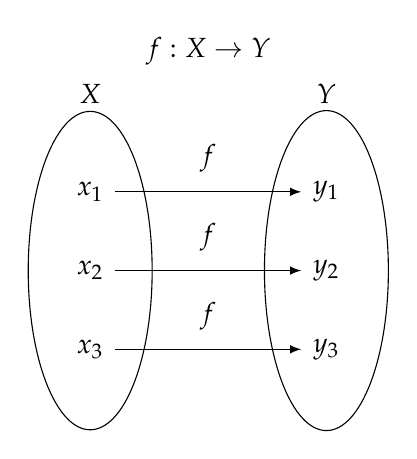
\begin{tikzpicture}[
            every node/.style={on grid},
            set/.style={circle,inner sep=2pt},
            every fit/.style={draw,ellipse,text width=25pt},
            >=latex
        ]
        
        % Draw domain %
        \node[set] (x1) {$x_1$};
        \node[set,below = of x1] (x2) {$x_2$};
        \node[set,below = of x2] (x3) {$x_3$};
        \node[above = of x1,anchor=south] (X) {$X$};

        % Draw co-domain %
        \node[set, right=3cm of x1] (y1) {$y_1$};
        \node[set, below = of y1] (y2) {$y_2$};
        \node[set, below = of y2] (y3) {$y_3$};
        \node[above = of y1,anchor=south] (Y) {$Y$};
        
        % Draw arrows %
        \draw[->] (x1) -- node[label=above:$f$] {} (y1);
        \draw[->] (x2) -- node[label=above:$f$] {} (y2);
        \draw[->] (x3) -- node[label=above:$f$] {} (y3);
        
        % Draw ellipses %
        \begin{pgfonlayer}{background}
            \node[fit = (x1) (x3) ] {};
            \node[fit = (y1) (y3) ] {};
        \end{pgfonlayer}

        % Label %
        \node[anchor=south] at (current bounding box.north) {$f:X \to Y$};
        \end{tikzpicture}
    \end{figure}

    \textbf{Examples: }
    \begin{itemize}
        \item $f: \N \to \N, f(n) = n!$ is a function
        \item $f: \R \to \R, f(x) = \ln{x}$ is not a function as $f(x)$ is 
        undefined for $x \lt 0$
        \item $f: \Q \to \N, f(\frac{n}{m}) = n$ is not a function as there are multiple
        ways to write the same input with different outputs, e.g. $\frac{3}{2} = 3$ but $\frac{6}{4} = 6$.
    \end{itemize}

    \subsubsection{Function Terminology}
    Let $f:X \to Y$ be a function. Then we say:
    \begin{itemize}
        \item $X$ is called the \textbf{domain} of $f$
        \item $Y$ is called the \textbf{co-domain} of $f$
        \item $f(x) \in Y$ is called the \textbf{image} of $X$ (also called range).\\
    \end{itemize}

    \begin{figure}[!hbt]
        \centering
        \begin{tikzpicture}[
            every node/.style={on grid},
            set/.style={circle,inner sep=2pt},
            every fit/.style={draw,ellipse,text width=25pt},
            >=latex
        ]
        
        % Draw domain %
        \node[set] (x1) {$x_1$};
        \node[set,below = of x2] (x3) {$x_3$};
        \node[above = of x1,anchor=south] (X) {$X$};

        % Draw co-domain and image of x %
        \node[set, right=3cm of x1] (cd1) {};
        \node[set, below= of cd1] (y1) {$f(x_1)$};
        \node[set, below= of y1] (y2) {$f(x_2)$};
        \node[set, below= of y2] (cd2) {};
        \node[above = of cd1,anchor=south] (Y) {$Y$};
        \node[above = of y1,anchor=south] (I) {Image};
        
        % Draw arrows %
        \draw[->] (x1) -- node[label=above:$f$] {} (y1);
        \draw[->] (x2) -- node[label=above:$f$] {} (y2);
        
        % Draw ellipses %
        \begin{pgfonlayer}{background}
            \node[fit = (x1) (x3) ] {};
            \node[fit = (cd1) (cd2), minimum width = 3cm, minimum height = 4cm] {};
            \node[fit = (y1) (y2)] {};
        \end{pgfonlayer}
        \end{tikzpicture}
    \end{figure}

    Similarly, the \textbf{pre-image} of a y is the set of all input values which
    map to the co-domain $Y$. This is written as 
    $f^{-1}(y)=\{x\in X \mid f(x) = y\} \subseteq X$. In essence, it explains where
    does $y$ come from under the function $f(x)$.

    \subsubsection{Identity Function}
    \begin{definition}[Identity Function]
        \label{def:identity-function}
        The \textbf{identity function} is a function which maps a set to iteself. For any set $S$,
        $i_x:X \to X$ is defined by $i_x(a) = a, a \in X$.       
    \end{definition}

    \subsubsection{Floors and Ceilings}
    \begin{definition}[Floor]
        \label{def:floor}
        For $x \in \R$, the floor of $x$ is the unique integer $n$ such that $n \le x \le n+1$.
        In essence, it is "rounding down" $x$ in terms of value. It is written as $\lfloor x \rfloor$. \\
    \end{definition}

    \begin{definition}[Ceiling]
        \label{def:ceiling}
        For $x \in \R$, the ceiling of $x$ is the unique integer $m$ such that $m-1 \le x \le m$.
        In essence, it is "rounding up" $x$ in terms of value. It is written as $\lceil x \rceil$.
    \end{definition}

    \textbf{Note: } both floor and ceiling are functions $f: \R \to \Z$. 
    Additionally, for $x \lt 0$, the rounding up/down of these functions are reversed.

    \textbf{Examples:}
    \begin{itemize}
        \item $\lfloor 2.5 \rfloor = 2$
        \item $\lfloor -2.5 \rfloor = -3$
        \item $\lceil 2.5 \rceil = 3$
        \item $\lceil -2.5 \rceil = -2$
    \end{itemize}

    \newpage
    \section{Week 3}

    \newpage
    \section{Week 4}

    \newpage
    \section{Week 5}
    
\end{document}